\caulc 
%%%============= EX_1 =============%%%
\begin{ex}%[1D3H2-3]%[TDMZZ08-1-TN]%[Mui Doan]
	Giới hạn $\lim\limits_{x \to +\infty} \left( \dfrac{4x^2 + 3}{x^2 - 1} \right)$ bằng
	\choice
	{$-3$}
	{$0$}
	{\True $4$}
	{$+\infty$}
	\loigiai{
		Ta có $\lim\limits_{x \to +\infty} \left( \dfrac{4x^2 + 3}{x^2 - 1}\right)=\lim\limits_{x \to +\infty}\dfrac{4 +\dfrac{3}{x^2}}{1 -\dfrac{1}{x^2}}=4$.
	}
\end{ex}

%%%============= EX_2 =============%%%
\begin{ex}%%[1H8H7-1]%[TDMZZ08-02][Huỳnh Trí Thiện]
	Thể tích của khối chóp có diện tích đáy bằng $6$ và chiều cao bằng $2$ là
	\choice
	{\True $V = 4$}
	{$V = 12$}
	{$6$}
	{$V = 24$}
	\loigiai{
		Thể tích của khối chóp là
		\[ V = \dfrac{1}{3}\cdot B\cdot h = \dfrac{1}{3} \cdot 6 \cdot 2 = 4. \]
		Vậy thể tích khối chóp bằng $4$.
	}
\end{ex}

%%%============= EX_3 =============%%%
\begin{ex}%[1D6N4-2]%[TDM21]
	Tập nghiệm của phương trình $\log_2(x^2 - 1) = 3$ là
	\choice
	{$\left\lbrace3\right\rbrace$}
	{\True $\left\lbrace\pm 3\right\rbrace$}
	{$\left\lbrace-3\right\rbrace$}
	{$\left\lbrace\pm\sqrt{7}\right\rbrace$}
	\loigiai{
		Điều kiện xác định $x^2 - 1 > 0 \Leftrightarrow \hoac{& x > 1 \\ & x < -1.}$\\
		Ta có
		\[ \log_2(x^2 - 1) = 3 \Leftrightarrow x^2 - 1 = 2^3 \Leftrightarrow x^2 - 1 = 8 \Leftrightarrow x^2 = 9 \Leftrightarrow x = \pm 3 \text{ (thỏa mãn điều kiện)}.\]
		Vậy tập nghiệm của phương trình là $S = \left\lbrace\pm 3\right\rbrace$.
	}
\end{ex}

%%%============= EX_4 =============%%%
\begin{ex}%[1D7N2-1]%[TDMZZ08]%[Nguyễn Tấn Linh]
	Đạo hàm của hàm số $y=\mathrm{e}^{3x}$ là
	\choice
	{$y'=\mathrm{e}^{3x}$}
	{\True $y'=3\cdot \mathrm{e}^{3x}$}
	{$y'=\dfrac{\mathrm{e}^{3x}}{3}$}
	{$y'=\mathrm{e}^{9x}$}
	\loigiai{
		Ta có $y'=(3x)'\cdot \mathrm{e}^{3x}=3\cdot \mathrm{e}^{3x}$.
	}
\end{ex}

%%%============= EX_5 =============%%%
\begin{ex}%[2D1N4-1]%[TDMZZ08]%[Phạm Hải Dương]
	Đường tiệm cận đứng của đồ thị hàm số $y = \dfrac{1}{2x - 3}$ là
	\choice
	{$x = 3$}
	{$y = \dfrac{1}{2}$}
	{$y = \dfrac{3}{2}$}
	{\True $x = \dfrac{3}{2}$}
	\loigiai{
		Tập xác định $\mathscr{D}=\mathbb{R}\setminus\left\{\dfrac{3}{2}\right\}$.\\
		Ta có $\lim\limits_{x\to\left(\frac{3}{2}\right)^\pm}\dfrac{1}{2x-3} =\pm\infty$.\\
		Vậy đường thẳng $x = \dfrac{3}{2}$ là đường tiệm cận đứng của đồ thị hàm số.
	}
\end{ex}

%%%============= EX_6 =============%%%
\begin{ex}%[2D1N2-1]%[TDMZZ08]%[Bồ Văn Hậu]
	Cho hàm số $y=f(x)$ có biểu thức đạo hàm $f'(x)=(x-1)(x^2-4x+3)$ với mọi $x \in \mathbb{R}$. Hỏi hàm số $y=f(x)$ có tất cả bao nhiêu điểm cực trị?
	\choice
	{$3$}
	{$2$}
	{\True $1$}
	{$0$}
	\loigiai{
		Tập xác định $\mathscr{D}=\mathbb{R}$.\\
		Ta có $f'(x)=0 \Leftrightarrow \hoac{&x-1=0\\&x^2-4x+3=0} \Leftrightarrow \hoac{&x=1\\ &x=1 \text{ hoặc } x=3.}$\\
		Bảng xét dấu $f'(x)$
		\begin{center}
			
\begin{tikzpicture}
				\tkzTabInit[espcl=2.5,lgt=1.5]
				{$x$/0.7,$f'(x)$/0.7}
				{$-\infty$,$1$,$3$,$+\infty$}
				\tkzTabLine{,-,0,-,0,+,}
			\end{tikzpicture}
		\end{center}
		Dựa vào bảng xét dấu, ta thấy $f'(x)$ đổi dấu $1$ lần qua điểm $x=3$ trên $\mathbb{R}$ nên hàm số $y = f(x)$ có đúng $1$ điểm cực trị.
	}
\end{ex}

%%%============= EX_7 =============%%%
\begin{ex}%[2H2H1-3]%[TDMZZ08]%[Nguyễn Sơn Thành]
	\immini[thm]{Cho hình lập phương $ABCD.A'B'C'D'$. Đáp án nhận xét \textbf{sai} là
		\choice
		{$\overrightarrow{AB} \cdot \overrightarrow{CC'} = 0$}
		{$\overrightarrow{AC} \cdot \overrightarrow{BD'} = 0$}
		{\True $\overrightarrow{AB'} \cdot \overrightarrow{A'D} = 0$}
		{$\overrightarrow{AB} \cdot \overrightarrow{B'C} = 0$}}{\begin{tikzpicture}[line cap=round, line join=round, font=\footnotesize, >=stealth, scale=.7]
			\path 
			(0,0) coordinate (A)
			(4,0) coordinate (D)
			(-2,-2) coordinate (B)
			($(D) - (A) + (B)$) coordinate (C)
			($(A) + (0,3)$) coordinate (A')
			($(B) + (0,3)$) coordinate (B')
			($(C) + (0,3)$) coordinate (C')
			($(D) + (0,3)$) coordinate (D')
			;
			\draw[dashed] (A')--(A) (B)--(A)--(D);
			\draw (A')--(B')--(C')--(D')--cycle (D')--(D)--(C) (B')--(B)--(C)--(C')--cycle;
			\foreach \i/\r in {A/180, B/-135, C/-45, D/0, A'/105, B'/180, C'/-45, D'/45}{
				\filldraw[black] (\i) circle (1pt);
				\draw (\i) circle (1pt);
				\node at ($(\i) + (\r:4mm)$) {$\i$};
			}
	\end{tikzpicture}}	
	\loigiai{
		Xét các phương án:
		\begin{itemize}
			\item Vì $CC' \perp (ABCD)$ nên $CC' \perp AB \Rightarrow \overrightarrow{AB} \cdot \overrightarrow{CC'} = 0$.
			\item Ta có $AC \perp BD$ và $AC \perp BB'$ nên $AC \perp (BDD'B')$.\\ 
			Mà $BD' \subset (BDD'B')$ nên $AC \perp BD' \Rightarrow \overrightarrow{AC} \cdot \overrightarrow{BD'} = 0$. 
			\item Sử dụng phương pháp tọa độ với cạnh bằng $1$, ta có $\overrightarrow{AB'} = (1; 0; 1)$ và $\overrightarrow{A'D} = (0; 1; -1)$.\\ 
			Khi đó $\overrightarrow{AB'} \cdot \overrightarrow{A'D} = 1 \cdot 0 + 0 \cdot 1 + 1 \cdot (-1) = -1 \ne 0$.
			\item Vì $AB \perp (BCC'B')$ nên $AB \perp B'C \Rightarrow \overrightarrow{AB} \cdot \overrightarrow{B'C} = 0$. 
		\end{itemize}
		Vậy nhận xét $\overrightarrow{AB'} \cdot \overrightarrow{A'D} = 0$ là nhận xét \textbf{sai}.
	}
\end{ex}

%%%============= EX_8 =============%%%
\begin{ex}%[2D4N1-31]%[TDMZZ08]%[Lê Phúc]
	Họ nguyên hàm của hàm số $f(x)=2x-\sin x$ là
	\choice
	{\True $x^2+\cos x+C$}
	{$x^2-\cos x+C$}
	{$2-\cos x+C$}
	{$2+\cos x+C$}
	\loigiai{
		Ta có $\displaystyle\int\limits f(x) \mathrm{\,d}x=\displaystyle\int\limits (2x-\sin x) \mathrm{\,d}x=x^2+\cos x+C$.
	}
\end{ex}

%%%============= EX_9 =============%%%
\begin{ex}%[2H5N3-2]%TDMZZ08-Trần Văn Thiện
	Trong không gian $Oxyz$, cho mặt cầu $(S)\colon x^2+y^2+z^2+2x+2y=0$. Tọa độ tâm của mặt cầu $(S)$ là
	\choice
	{\True $(-1;-1;0)$}
	{$(1;1;0)$}
	{$(0;1;0)$}
	{ $(2;2;-2023)$}
	\loigiai{ 
		Mặt cầu $(S)\colon x^2+y^2+z^2+2x+2y=0$ có tâm là $I(-1;-1;0)$.
	}
\end{ex}

%%%============= EX_10 =============%%%
\begin{ex}%[0D0H2-2]%[TDMZZ08]%[Đình Nguyên]
	Gieo một con súc sắc cân đối đồng chất $2$ lần liên tiếp. Tính xác suất để tổng số chấm xuất hiện trong $2$ lần gieo là một số tự nhiên chia hết cho $5$?
	\choice
	{$\dfrac{1}{9}$}
	{\True $\dfrac{7}{36}$}
	{$\dfrac{1}{12}$}
	{$\dfrac{1}{6}$}
	\loigiai{
		Số phần tử của không gian mẫu là $n(\Omega) = 6 \cdot 6 = 36$.
		\begin{itemize}
			\item Gọi $A$ là biến cố: \lq\lq Tổng số chấm xuất hiện trong $2$ lần gieo là một số tự nhiên chia hết cho $5$\rq\rq.
			\item Vì số chấm trên mỗi mặt thuộc tập $\{1; 2; 3; 4; 5; 6\}$ nên tổng số chấm $S$ trong $2$ lần gieo thỏa mãn $2 \le S \le 12$.
			\item Các giá trị của $S$ chia hết cho $5$ là $S \in \{5; 10\}$.
			\begin{itemize}
				\item Trường hợp $1$: $S = 5 \Rightarrow$ có các kết quả $\{(1; 4); (4; 1); (2; 3); (3; 2)\}$. Có $4$ kết quả.
				\item Trường hợp $2$: $S = 10 \Rightarrow$ có các kết quả $\{(4; 6); (6; 4); (5; 5)\}$. Có $3$ kết quả.
			\end{itemize}
			\item Số kết quả thuận lợi cho biến cố $A$ là $n(A) = 4 + 3 = 7$.
		\end{itemize}
		Vậy xác suất cần tìm là $\mathrm{P}(A) = \dfrac{n(A)}{n(\Omega)} = \dfrac{7}{36}$.
	}
\end{ex}

%%%============= EX_11 =============%%%
\begin{ex}%%[2D1H4-3]%[TDMZZ08]%[Huynh Quốc Đạt]
	Số đường tiệm cận ngang của đồ thị hàm số $y = \dfrac{\sqrt{x^2+1}+x}{x-1}$ là
	\choice
	{$3$}
	{\True $2$}
	{$1$}
	{$0$}
	\loigiai{
		Tập xác định của hàm số là $\mathscr{D} = \mathbb{R} \setminus \{1\}$.\\
		Để tìm tiệm cận ngang, ta xét giới hạn của hàm số khi $x \to +\infty$ và $x \to -\infty$.
		\begin{itemize}
			\item Ta có
			\[\lim_{x \to +\infty} \dfrac{\sqrt{x^2+1}+x}{x-1} = \lim_{x \to +\infty} \dfrac{x\left(\sqrt{1+\tfrac{1}{x^2}}+1\right)}{x\left(1-\tfrac{1}{x}\right)} = \lim_{x \to +\infty} \dfrac{\sqrt{1+\tfrac{1}{x^2}}+1}{1-\tfrac{1}{x}} = \dfrac{1+1}{1} = 2.\]
			Suy ra đường thẳng $y = 2$ là một tiệm cận ngang.
			\item Ta có 
			\begin{align*}
				\lim_{x \to -\infty} \dfrac{\sqrt{x^2+1}+x}{x-1} &= \lim_{x \to -\infty} \dfrac{|x|\sqrt{1+\tfrac{1}{x^2}}+x}{x-1} = \lim_{x \to -\infty} \dfrac{-x\sqrt{1+\tfrac{1}{x^2}}+x}{x-1} \\
				&= \lim_{x \to -\infty} \dfrac{-x\left(\sqrt{1+\tfrac{1}{x^2}}-1\right)}{x\left(1-\tfrac{1}{x}\right)} = \lim_{x \to -\infty} \dfrac{-\sqrt{1+\tfrac{1}{x^2}}+1}{1-\tfrac{1}{x}} = \dfrac{-1+1}{1} = 0.
			\end{align*}
			Suy ra đường thẳng $y = 0$ là một tiệm cận ngang.
		\end{itemize}
		Vậy đồ thị hàm số đã cho có $2$ đường tiệm cận ngang.
	}
\end{ex}

%%%============= EX_12 =============%%%
\begin{ex}%[2H5V2-6]%[TDMZZ08]%[Nguyễn Trí Minh Tuấn]
	Trong không gian $Oxyz$, cho đường thẳng $d \colon \dfrac{x-1}{3}=\dfrac{y-2}{-1}=\dfrac{z+2}{2}$ và điểm $A(-1;2;0)$. Hình chiếu vuông góc của điểm $A$ lên đường thẳng $d$ có hoành độ là
	\choice
	{$\dfrac{15}{7}$}
	{\True $\dfrac{4}{7}$}
	{$-\dfrac{16}{7}$}
	{$-\dfrac{1}{7}$}
	\loigiai{
		Đường thẳng $d$ có một vectơ chỉ phương $\overrightarrow{u}=(3;-1;2)$.\\
		Gọi $H$ là hình chiếu vuông góc của $A(-1;2;0)$ lên $d$.\\ 
		Khi đó $H\in d$, nên $H(1+3t;\,2-t;\,-2+2t)$, suy ra $\overrightarrow{AH}=(2+3t;-t;-2+2t)$.\\
		Vì $AH\perp d$ nên 
		\begin{align*}
			&\overrightarrow{AH}\cdot \overrightarrow{u}=0\\
			\Leftrightarrow \quad &3(2+3t)+(-1)(-t)+2(-2+2t)=0\\
			\Leftrightarrow \quad &6+9t+t-4+4t=0\\
			\Leftrightarrow \quad &2+14t=0\\
			\Leftrightarrow \quad &t =-\dfrac{1}{7}.
		\end{align*}
		Suy ra hoành độ của $H$ là $x_H=1+3t=1+3\left(-\dfrac{1}{7}\right)=\dfrac{4}{7}$.
	}
\end{ex}

\cauds
%%%============= EX_13 =============%%%
\begin{ex}%[1D6V4-5]%[TDMZZ08]%[Dương Công Tạo]
	Cho hàm số $f(x) = 2^{2x} - 3x-1$.
	\choiceTF
	{Tập xác định của hàm số là $(0;+\infty)$}
	{\True $f'(x) = 2^{2x+1} \ln 2-3$}
	{\True $f''(x) = 2^{2x+2} \ln^2 2$}
	{\True $f(x) \le 0 \Leftrightarrow 0 \le x \le 1$}
	\loigiai{
		\begin{itemchoice}
			\itemch Tập xác định của hàm số $f(x) = 2^{2x} - 3x-1$ là $\mathscr{D}=\mathbb{R}$.
			\itemch Ta có $f'(x) = 2\cdot 2^{2x}\cdot\ln 2 - 3= 2^{2x+1}\cdot\ln 2 - 3$.
			\itemch Ta có $f''(x)= 2\cdot 2^{2x+1}\cdot\ln 2\cdot\ln 2 = 2^{2x+2} \ln^2 2$.
			\itemch Xét bất phương trình $f(x) \le 0$ hay $2^{2x} - 3x-1\le 0$.\\
			Ta có $f(0)=0$ và $f(1)= 0$.\quad(1)\\
			Mà $f''(x) = 2^{2x+2} \ln^2 2 > 0$ với mọi $x$.\quad(2) \\
			Từ (1) và (2) suy ra phương trình $f(x) = 0$ có tối đa $2$ nghiệm. \\
			Ở đây ta đã tìm ra đúng $2$ nghiệm là $x=0$ và $x=1$.\\
			Vì đồ thị hàm số $f(x)$ có bề lõm hướng lên (do $f''(x)>0$), nên giá trị của hàm số sẽ nhỏ hơn hoặc bằng $0$ trong đoạn giữa hai nghiệm.\\
			Vậy $f(x) \le 0 \Leftrightarrow x \in [0; 1]$.
		\end{itemchoice}
	}
\end{ex}

%%%============= EX_14 =============%%%
\begin{ex}%[2D4V3-2]%[TDMZZ08]%[Văn Minh Thoại]
	\immini[thm]{Trên một mảnh đất hình vuông $ABCD$ có cạnh bằng $60$ mét người ta muốn trồng hoa trong phần tô màu được giới hạn bởi một phần đồ thị của hàm bậc ba và cạnh $AB$. Biết rằng $DE=45$ mét. Ta tiến hành gắn hệ trục toạ độ $Oxy$ với đơn vị dài trên mỗi trục là mét, trục $Ox$ hướng theo vectơ $\overrightarrow{AB}$, trục $Oy$ hướng theo vectơ $\overrightarrow{AD}$. Phương trình đường cong trong hình là $y=f(x)=ax^3+bx^2+cx+d$.}{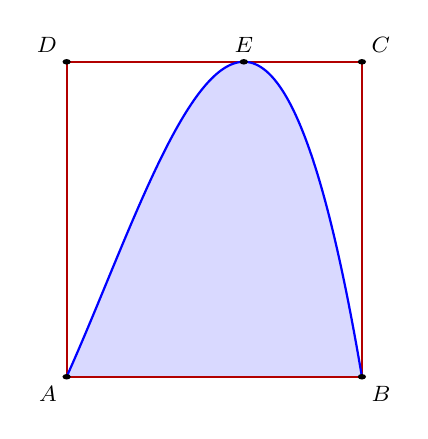
\begin{tikzpicture}[scale=1, font=\footnotesize, line join=round, line cap=round, >=stealth, xscale=1.5]
			\def\xmin{1.5}
			\def\xmax{4}
			\def\ymin{0}
			\def\ymax{4}
			\fill[blue!15]
			(1.5, 0) -- plot[smooth, samples=200, domain=1.5:\xmax]
			(\x, {(-8/9)*(\x)^3+(44/9)*(\x)^2-(16/3)*(\x)}) -- (4, 0) -- cycle; 
			\draw[red!70!black, thick] (1.5, 0)--(4, 0)--(4, 4)--(1.5, 4)--cycle; 
			\draw[blue, thick, smooth, samples=200, domain=1.5:\xmax]
			plot (\x, {(-8/9)*(\x)^3+(44/9)*(\x)^2-(16/3)*(\x)}); 
			\fill (1.5, 0) circle (1pt) node[below left] {$A$}
			(4, 0) circle (1pt) node[below right] {$B$}
			(4, 4) circle (1pt) node[above right] {$C$}
			(1.5, 4) circle (1pt) node[above left] {$D$}
			(3, 4) circle (1pt) node[above] {$E$}; 
	\end{tikzpicture}}
	\choiceTF
	{\True $E(45; 60)$}
	{\True $d=0$}
	{$6070a+90b+c=0$}
	{Diện tích phần tô màu trong hình vẽ tính theo mét vuông là $2\, 954$ m$^2$ \textit{(làm tròn kết quả đến hàng đơn vị)}}
	\loigiai{
		Gắn hệ trục tọa độ $Oxy$ với gốc tọa độ $O$ trùng với $A(0; 0)$. \\
		Vì $ABCD$ là hình vuông cạnh $60$ nên ta có tọa độ các đỉnh là $B(60; 0)$, $D(0; 60)$ và $C(60; 60)$.
		\begin{center}
			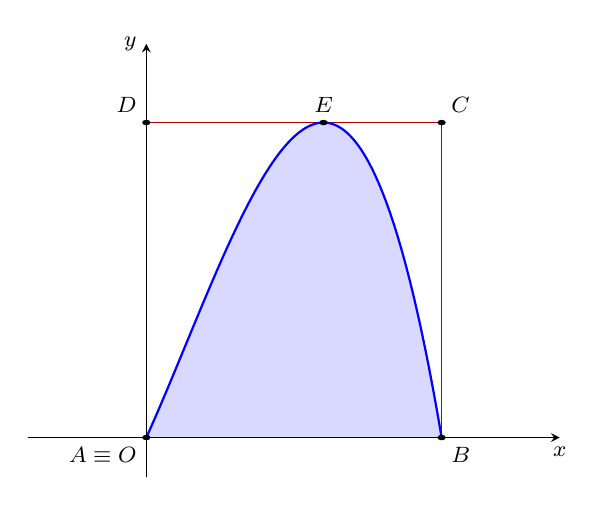
\begin{tikzpicture}[scale=1, font=\footnotesize, line join=round, line cap=round, >=stealth, xscale=1.5]
				\def\xmin{1.5}
				\def\xmax{4}
				\def\ymin{0}
				\def\ymax{4}
				\fill[blue!15]
				(1.5, 0) -- plot[smooth, samples=200, domain=1.5:\xmax]
				(\x, {(-8/9)*(\x)^3+(44/9)*(\x)^2-(16/3)*(\x)}) -- (4, 0) -- cycle; 
				\draw[red!70!black] (1.5, 0)--(4, 0)--(4, 4)--(1.5, 4)--cycle; 
				\draw[blue, thick, smooth, samples=200, domain=1.5:\xmax]
				plot (\x, {(-8/9)*(\x)^3+(44/9)*(\x)^2-(16/3)*(\x)}); 
				\draw[->] (0.5, 0)--(5, 0) node[below] {$x$}; 
				\draw[->] (1.5, -0.5)--(1.5, 5) node[left] {$y$}; 
				\fill (1.5, 0) circle (1pt) node[below left] {$A\equiv O$}
				(4, 0) circle (1pt) node[below right] {$B$}
				(4, 4) circle (1pt) node[above right] {$C$}
				(1.5, 4) circle (1pt) node[above left] {$D$}
				(3, 4) circle (1pt) node[above] {$E$}; 
			\end{tikzpicture}
		\end{center}
		\begin{itemchoice}
			\itemch Trục $Oy$ hướng theo $\overrightarrow{AD}$ nên $D$ nằm trên trục $Oy$. \\
			Điểm $E$ nằm trên đoạn $CD$ và cách $D$ một khoảng $DE=45$. \\
			Do đó hoành độ của $E$ là $45$, tung độ bằng với tung độ điểm $D$ là $60$. \\
			Vậy $E(45; 60)$.
			\itemch Đồ thị hàm số $f(x)$ đi qua gốc tọa độ $A(0; 0)$, thay $x=0$, $y=0$ vào phương trình hàm số ta được $f(0)=d=0$.
			\itemch Điểm $E(45; 60)$ là điểm cực đại của đồ thị hàm số nên $f'(45)=0$. \\
			Ta có đạo hàm $f'(x)=3ax^2+2bx+c$. \\
			Thay $x=45$ ta được $f'(45)=3a\cdot 45^2+2b\cdot 45+c=6\, 075a+90b+c=0$.
			\itemch Đồ thị đi qua điểm $B(60; 0)$ nên
			\begin{align*}
				&f(60)=0\\
				\Leftrightarrow \quad &a\cdot 60^3+b\cdot 60^2+c\cdot 60=0\\
				\Leftrightarrow \quad &3\, 600a+60b+c=0.
			\end{align*}
			Đồ thị đi qua điểm $E(45; 60)$ nên
			\begin{align*}
				&f(45)=60\\
				\Leftrightarrow \quad &a\cdot 45^3+b\cdot 45^2+c\cdot 45=60\\
				\Leftrightarrow \quad &91\, 125a+2\, 025b+45c=60.
			\end{align*}
			Từ các giả thiết, ta lập được hệ phương trình
			\[\heva{& 3\, 600a+60b+c=0\\& 6\, 075a+90b+c=0\\& 91\, 125a+2\, 025b+45c=60}\Leftrightarrow\heva{& a=-\dfrac{8}{2\, 025}\\& b=\dfrac{44}{135}\\& c=-\dfrac{16}{3}.}\]
			Vậy hàm số có phương trình là $f(x)=-\dfrac{8}{2\, 025}x^3+\dfrac{44}{135}x^2-\dfrac{16}{3}x$. \\
			Diện tích phần tô màu giới hạn bởi đồ thị $f(x)$ và trục $Ox$ là
			\[S=\displaystyle\int\limits_{0}^{60}\left(-\dfrac{8}{2\, 025}x^3+\dfrac{44}{135}x^2-\dfrac{16}{3}x\right)\mathrm{\,d}x=\dfrac{3\, 200}{3}\approx 1\, 067\text{ (m}^2\text{)}. \]
		\end{itemchoice}
	}
\end{ex}

%%%============= EX_15 =============%%%
\begin{ex}%[2H5V2-8]%[TDMZZ08]%[Vũ Hồng Toàn]
	Trong không gian $Oxyz$ có đơn vị dài trên mỗi trục là kilômét, một máy bay đang ở vị trí $A(2;-2;1)$ và sẽ hạ cánh tại điểm $B(4;3;0)$ trên đường băng $MN$. Mặt đất là mặt phẳng $(Oxy)$. Một đám mây được mô tả bởi mặt phẳng $(\alpha)\colon x-y+10z-4=0$.
	\choiceTF
	{\True Phương trình chính tắc của đường thẳng $AB$ là $\dfrac{x-2}{2} = \dfrac{y+2}{5} = \dfrac{z-1}{-1}$}
	{Góc trượt của máy bay (giữa đường bay $AB$ với mặt nằm ngang) bằng $15^\circ$ (\textit{làm tròn kết quả đến hàng đơn vị})}
	{Máy bay gặp đám mây tại điểm $(a;b;c)$ có $a+b+c=3$}
	{Theo quy định an toàn hạ cánh, ở độ cao tối thiểu $120$\,m thì phi công phải nhìn thấy điểm $M(4;1{,}5;0)$. Biết tầm nhìn của phi công là $980$\,m. Nếu giữ hướng bay $AB$ thì phi công với chiếc máy bay này sẽ không đúng quy định an toàn hạ cánh}
	\loigiai{
		\begin{itemchoice}
			\itemch Đường thẳng $AB$ đi qua $A(2; -2; 1)$ và có vectơ chỉ phương $\overrightarrow{u}=\overrightarrow{AB} = (2; 5; -1)$ nên có phương trình chính tắc là $\dfrac{x-2}{2} = \dfrac{y+2}{5} = \dfrac{z-1}{-1}$.
			\itemch Mặt phẳng nằm ngang $(Oxy)$ có phương trình $z=0$ nên có vectơ pháp tuyến \break$\overrightarrow{n} = (0; 0; 1)$.\\ 
			Gọi $\varphi$ là góc giữa đường bay $AB$ và mặt phẳng $(Oxy)$, ta có
			\begin{align*}
				\sin \varphi = \dfrac{\left|\overrightarrow{u} \cdot \overrightarrow{n}\right|}{\left|\overrightarrow{u}\right| \cdot \left|\overrightarrow{n}\right|} = \dfrac{|2 \cdot 0 + 5 \cdot 0 + (-1) \cdot 1|}{\sqrt{2^2+5^2+(-1)^2} \cdot \sqrt{0^2+0^2+1^2}} = \dfrac{1}{\sqrt{30}}.
			\end{align*}
			Suy ra $\varphi \approx 11^\circ$.
			\itemch Gọi $C=AB\cap (\alpha)$.\\
			Vì $C\in AB\Rightarrow C(2+2t;-2+5t;1-t)$.\\
			Mặt khác $C\in (\alpha)\colon x-y+10z-4=0$ nên
			\begin{align*}
				&(2+2t) - (-2+5t) + 10(1-t) - 4 = 0\\
				\Rightarrow\quad & t=\dfrac{10}{13}.
			\end{align*}
			Suy ra $C\left(\dfrac{46}{13};\dfrac{24}{13};\dfrac{3}{13}\right)$.\\
			Khi đó $a=\dfrac{46}{13}$; $b=\dfrac{24}{13}$; $c=\dfrac{3}{13}$.\\
			Do đó $a+b+c=\dfrac{46+24+3}{13}=\dfrac{73}{13}\ne 3$.
			\itemch Ta có $120$\,m $= 0{,}12$\,km; $980$\,m $= 0{,}98$\,km.\\
			Độ cao tối thiểu $120$\,m tương ứng với $z = 0{,}12$\,km.\\
			Suy ra $1-t = 0{,}12 \Rightarrow t = 0{,}88$.\\
			Tại $t = 0{,}88$, vị trí máy bay là $P(3{,}76; 2{,}4; 0{,}12)$.\\
			Khoảng cách từ máy bay $P$ đến điểm $M(4; 1{,}5; 0)$ là
			\[PM = \sqrt{(4-3{,}76)^2 + (1{,}5-2{,}4)^2 + (0-0{,}12)^2} = \sqrt{0{,}882} \approx 0{,}939\text{ (km)} = 939\text{ (m)}.\]
			Vì $PM \approx 939$\,m$< 980$\,m nên điểm $M$ nằm trong tầm nhìn của phi công, do đó phi công sẽ nhìn thấy được điểm $M$.\\
			Suy ra chiếc máy bay này đạt quy định an toàn hạ cánh.
		\end{itemchoice}
	}
\end{ex}

%%%============= EX_16 =============%%%
\begin{ex}%[2D6C2-4]%[TDMZZ08]%[Hà Văn Hảo]
	Có hai hộp đựng các viên bi có cùng kích thước và khối lượng. Hộp I đựng $3$ bi đỏ $6$ bi xanh, hộp II đựng $4$ bi đỏ và $5$ bi xanh. Chọn ngẫu nhiên một hộp để tiến hành lấy ngẫu nhiên liên tiếp (không hoàn lại) hai lần mỗi lần một viên bi. Gọi $B$ là biến cố chọn được hộp I, $A$ là biến cố lần thứ nhất lấy được bi đỏ, $C$ là biến cố lần thứ hai lấy được bi đỏ. 
	\choiceTF
	{\True $\mathrm{P}(B) = \dfrac{1}{2}$}
	{\True $\mathrm{P}\left(C \mid B\right) = \dfrac{1}{3}$ và $\mathrm{P}\left(A \mid \overline{B}\right) = \dfrac{4}{9}$}
	{\True $\mathrm{P}\left(C \mid \overline{B}\right) = \dfrac{4}{9}$}
	{\True $\mathrm{P}(C) = \dfrac{7}{18}$}
	\loigiai{
		\begin{itemchoice}
			\itemch Vì chọn ngẫu nhiên một trong hai hộp nên xác suất chọn được mỗi hộp là bằng nhau.\\
			Do đó, $\mathrm{P}(B) = \mathrm{P}\left(\overline{B}\right) = \dfrac{1}{2}$.
			\itemch Tính $\mathrm{P}\left(A \mid \overline{B}\right)$ và $\mathrm{P}\left(C \mid B\right)$:
			\begin{itemize}
				\item Xét biến cố có điều kiện $\mathrm{P}\left(A \mid \overline{B}\right)$.\\
				Đây là xác suất lấy được bi đỏ ở lần thứ nhất khi biết đã chọn hộp II.\\
				Hộp II có $4$ đỏ và $5$ xanh (tổng $9$ viên), nên $\mathrm{P}\left(A \mid \overline{B}\right) = \dfrac{4}{9}$.
				\item Xét biến cố có điều kiện $\mathrm{P}\left(C \mid B\right)$.\\
				Đây là xác suất lấy được bi đỏ ở lần thứ hai khi biết đã chọn hộp I.\\
				Sử dụng công thức xác suất toàn phần trong không gian của hộp I.
				\begin{align*}
					\mathrm{P}\left(C \mid B\right) &= \mathrm{P}\left(C \mid A \cap B\right) \cdot \mathrm{P}\left(A \mid B\right) + \mathrm{P}\left(C \mid \overline{A} \cap B\right) \cdot \mathrm{P}\left(\overline{A} \mid B\right) \\
					&= \dfrac{2}{8} \cdot \dfrac{3}{9} + \dfrac{3}{8} \cdot \dfrac{6}{9} \\
					&= \dfrac{1}{3}.
				\end{align*}
			\end{itemize}
			\itemch Xét biến cố có điều kiện $\mathrm{P}\left(C \mid \overline{B}\right)$.\\
			Sử dụng công thức xác suất toàn phần trong không gian của hộp II.
			\begin{align*}
				\mathrm{P}\left(C \mid \overline{B}\right) &= \mathrm{P}\left(C \mid A \cap \overline{B}\right) \cdot \mathrm{P}\left(A \mid \overline{B}\right) + \mathrm{P}\left(C \mid \overline{A} \cap \overline{B}\right) \cdot \mathrm{P}\left(\overline{A} \mid \overline{B}\right) \\
				&= \dfrac{3}{8} \cdot \dfrac{4}{9} + \dfrac{4}{8} \cdot \dfrac{5}{9} \\
				&= \dfrac{4}{9}.
			\end{align*}
			\itemch Để tính $\mathrm{P}(C)$, ta sử dụng công thức xác suất toàn phần dựa trên việc chọn hộp
			\[ \mathrm{P}(C) = \mathrm{P}\left(C \mid B\right) \cdot \mathrm{P}(B) + \mathrm{P}\left(C \mid \overline{B}\right) \cdot \mathrm{P}\left(\overline{B}\right). \]
			Thay vào công thức ta được
			\[ \mathrm{P}(C) = \dfrac{1}{3} \cdot \dfrac{1}{2} + \dfrac{4}{9} \cdot \dfrac{1}{2} = \dfrac{1}{6} + \dfrac{2}{9} = \dfrac{3}{18} + \dfrac{4}{18} = \dfrac{7}{18}. \]
		\end{itemchoice}
	}
\end{ex}

\caukq
%%%============= EX_17 =============%%%
\begin{ex}%[0D2V2-3]%[TDMZZ08]%[Võ Hiệp]
	Một cửa hàng có kế hoạch nhập về hai loại máy tính A và B, giá mỗi chiếc của loại A và loại B lần lượt là $10$ triệu đồng và $15$ triệu đồng với số vốn ban đầu không vượt quá $4$ tỉ đồng. Bán được một máy loại A thu lợi nhuận $3$ triệu đồng, bán được một máy loại B thu được lợi nhuận $4$ triệu đồng. Cửa hàng ước tính rằng tổng nhu cầu hằng tháng sẽ không vượt quá được $300$ máy. Hỏi để thu được lợi nhuận lớn nhất thì số máy loại B bán được sẽ nhiều hơn số máy loại A bán được là bao nhiêu?
	\par 
	\shortans[0]{100}
	\loigiai{
		Gọi $x$, $y$ lần lượt là số máy tính loại A và loại B mà cửa hàng nhập về ($x$, $y \in \mathbb{N}$). Khi đó
		\begin{itemize}
			\item Tổng số máy nhập về (cả hai loại máy tính) là $x+y$ (máy).
			\item Tổng số tiền nhập cả hai loại máy tính là $10x+15y$ (triệu đồng).
		\end{itemize}
		Lợi nhuận thu được là $F(x; y) = 3x + 4y$ (triệu đồng).\\
		Theo đề bài ta có hệ bất phương trình $\heva{&x + y \le 300 \\ &10x + 15y \le 4\,000 \\ &x \ge 0 \\ &y \ge 0 .}$\\	
		Biểu diễn miền nghiệm của hệ bất phương trình trên mặt phẳng tọa độ $Oxy$.
		Ta được là miền tứ giác $OABC$ (kể cả biên) với $O(0; 0)$, $A(300; 0)$, $B(100; 200)$, $C\left(0; \dfrac{800}{3}\right)$ như hình vẽ.
		\immini{
			\begin{itemize}
				\item Tại điểm $O(0;0)$.\\ Ta có $F(0;0)=3\cdot 0+ 4\cdot 0=0$.
				\item Tại điểm $A(300;0)$.\\ Ta có $F(300;0)=3\cdot 300+ 4\cdot 0=900$.
				\item Tại điểm $B(100;200)$.\\ Ta có $F(100;200)=3\cdot 100+ 4\cdot 200=1\,100$.
				\item Tại điểm $C\left(0; \dfrac{800}{3}\right)$. Chọn $y=266$ (vì $y\in\mathbb{N}$).\\ 
				Ta có $F(0;266)=3\cdot 0 + 4\cdot 266=1\,064$.
			\end{itemize}
		}{
			\begin{tikzpicture}[scale=1.3, font=\footnotesize, >=stealth]
				\draw[->] (-.5,0) -- (4.5,0) node[below] {$x$};
				\draw[->] (0,-.5) -- (0,3.5) node[left] {$y$};
				\draw[pattern=north east lines] (0,0) -- (3,0) -- (1,2) -- (0,8/3) -- cycle;
				\draw[smooth,samples=300] plot[domain=-.5:3.5](\x,{-(\x)+3});
				\draw[smooth,samples=300] plot[domain=-.5:4.5](\x,{-2/3*(\x)+8/3});
				\path 	
				(0,0) coordinate (O)
				(3,0) coordinate (A)
				(1,2) coordinate (B)
				(0,8/3) coordinate (C)
				;
				\foreach \x/\g in {O/-135,A/60,B/60,C/-150}\fill[black] (\x) circle (1pt) ($(\g:2mm)+(\x)$) node {$\x$};
				\node at (A) [below left] {$300$};
				\draw[fill=black] (0,3) circle (1pt) (0,3) node[right]{$300$};
				\draw[dashed]  (1,0)node[below]{$100$}|-(0,2) node[left]{$200$};
				\node[rotate=-45, shift={(45:.25)} ]at (2.2,.8) {$x+y=300$};
				\node[rotate=-35, shift={(35:.3)} ]at (3,.67) {$10x+15y=4\,000$};
			\end{tikzpicture}		
		}
		\noindent
		So sánh các giá trị trên, ta thấy lợi nhuận lớn nhất là $1\,100$ triệu đồng khi $x = 100$ và $y = 200$.\\ 
		Số máy loại B nhiều hơn số máy loại A là $200 - 100 = 100$ máy.
	}
\end{ex}

%%%============= EX_18 =============%%%
\begin{ex}%[2D4H2-6]%[TDMZZ08]%[Lê Hồ Quang Minh]
	Trong không gian $Oxyz$ có đơn vị dài trên mỗi trục là mét với mặt đất là mặt phẳng tọa độ $(Oxy)$, có một vật được coi như một hạt đang ở điểm $A(300;150;0)$ thì bắt đầu chuyển động thẳng theo hướng vectơ $\overrightarrow{u}=(2;2;1)$ đến điểm $B$ trong khoảng thời gian $30$ giây, với tốc độ $v(t)=0{,}3t^2$ (m/s), từ $B$ vật chuyển động tròn quanh điểm $I$ (với điểm $I$ đối xứng với $B$ qua mặt phẳng $(Oyz)$), trong khi chuyển động tròn độ cao của vật không đổi và tại $B$ vectơ vận tốc hướng theo chiều dương của trục $Oy$. Ngay khi vật đập vào mặt phẳng tọa độ $(Oyz)$ tại điểm $C$ thì nó bị dừng lại và rơi xuống đất ở điểm $D$. Hãy tính theo đơn vị mét tổng độ dài hành trình chuyển động từ $A$ đến $D$ của vật \textit{(làm tròn kết quả đến hàng đơn vị)}.
	\par
	\shortans[0]{7998}
	\loigiai{
		\begin{center}
			\begin{tikzpicture}[scale=1.1, line join=round, line cap=round, >=stealth]
				% 1. Vẽ hệ trục tọa độ Oxyz màu đỏ
				\draw[->, red, thick] (0,0) -- (8,0) node[below left, black] {$y$};
				\draw[->, red, thick] (0,0) -- (0,5) node[right, black] {$z$};
				\draw[->, red, thick] (0,0) -- (-2.5,-3) node[right, black] {$x$};
				\fill[yellow, draw=black] (0,0) circle (2pt);
				\coordinate (I) at (4.5, 4.2);
				\coordinate (B) at (1, 1.5);
				\coordinate (H) at (2.75, 2.85);
				\coordinate (C) at (6.5, 2.85);
				\coordinate (A) at (-0.5, -2);
				\coordinate (D) at (6.5, 0);
				\draw[green!50!black, thick] (B) to[bend right=10] (C);
				\draw[blue, ultra thick] (A) -- (B);
				\draw[blue, ultra thick] (B) -- (H);
				\draw[blue, ultra thick] (H) -- (C);
				\draw[blue, ultra thick] (C) -- (D);
				\draw[blue, dashed, thick] (H) -- (I) -- (C);
				\draw[->, black!70, thick] (B) -- (2.5, 1.5);
				\node[rotate=40, scale=0.7] at (1.87, 2.17) {//};
				\node[rotate=40, scale=0.7] at (3.62, 3.52) {//};
				\foreach \p/\l/\pos in {A/A/left, B/B/above left, H/H/above left, I/I/above, C/C/above right, D/D/below} {
					\fill (\p) circle (1pt);
					\node[\pos] at (\p) {$\l$};
				}
				\fill (0,0) circle (1pt);
				
			\end{tikzpicture}
		\end{center}
		Quãng đường vật đi được từ $A$ đến $B$ là 
		\[AB = \displaystyle \int\limits_0^{30} v(t) \mathrm{\,d}t = \int\limits_0^{30} 0{,}3t^2 \mathrm{\,d}t = 2\,700\text{ (m).}\]
		Ta có $\overrightarrow{AB} = \dfrac{AB}{\left|\overrightarrow{u}\right|} \cdot \overrightarrow{u} = \dfrac{2\,700}{3}\cdot (2; 2; 1) = (1\,800; 1\,800; 900) \Rightarrow B(2\,100; 1\,950; 900)$.\\
		Vì vật chuyển động tròn và có độ cao không đổi nên khi chuyển động từ $B$ đến $C$ là một cung tròn có tâm $I$, bán kính $IB = 2\mathrm{d}\big(B; (Oyz)\big) = 4\,200$.\\
		Độ dài quãng đường vật đi được từ lúc bắt đầu đến khi chạm mặt đất là
		\[S = AB + l_{\wideparen{BC}} + CD.\]
		Gọi $H$ là hình chiếu của $B$ trên mặt phẳng $(Oyz)$.\\
		Xét tam giác $IHC$ vuông tại $H$ có $\cos \widehat{HIC} = \dfrac{HI}{IC} = \dfrac{1}{2} \Rightarrow \widehat{HIC} = \dfrac{\pi}{3}$.\\
		Suy ra quãng đường từ $B$ đến $C$ là $l_{\wideparen{BC}} = \dfrac{\pi}{3} \cdot R = 1\,400\pi$ (m).\\
		Quãng đường từ $C$ đến $D$ là $CD = z_C = z_B = 900$ (m).\\
		Vậy tổng độ dài quãng đường vật đi được từ lúc bắt đầu đến khi chạm mặt đất là
		\[S = 2\,700 + 1\,400\pi + 900 = 3\,600 + 1\,400\pi \approx 7\,998 \text{ (m).}\]
	}
\end{ex}

%%%============= EX_19 =============%%%
\begin{ex}%[1H8V7-4]%[TDMZZ08]%[Duong Xuan Loi]
	Cho hình lăng trụ $ABC.A'B'C'$ có đáy $ABC$ là tam giác vuông tại $A$ với $AB=8$, $AC=12$, có $ABB'A'$ là hình thoi với $\widehat{AA'B'}=120^\circ$. Gọi $M$ là trung điểm của cạnh $BC$, có $C'M = 4\sqrt{3}$. Hãy tính thể tích của khối lăng trụ $ABC.A'B'C'$ \textit{(làm tròn kết quả đến hàng đơn vị)}.
	\par
	\shortans[0]{300}
	\loigiai{
		\immini{
			Gọi $N$ là trung diểm của $AB$.\\
			Ta có $ABB'A'$ là hình thoi với $\widehat{AA'B'}=120^\circ$ suy ra $\widehat{A'AB}=60^\circ$ nên $\triangle A'AB$ là tam giác đều.\\
			Suy ra $\heva{& A'N=4\sqrt{3} \\ & A'N\perp AB.}$\\
			Do đó  $\heva{& A'N\perp AB \\ & A'B'\parallel AB}\Rightarrow A'N\perp A'B' $.\\
			Mặt phẳng đáy $(A'B'C')$ vuông tại $A'$ nên $A'B'\perp A'C'$, do đó $A'B'\perp(A'C'N)$.\\
			Mặt khác $AB \parallel A'B'$ nên $AB \perp (A'C'N) \Rightarrow (ABC) \perp (A'C'N)$.
		}{
			\begin{tikzpicture}[scale=1, font=\footnotesize, line join=round, line cap=round,>=stealth]
				\path
				(0,0)coordinate (A)
				(2.3,-1.5)coordinate (B)
				(4,0)coordinate (C)
				($(A)+(-0.8,-3.2)$) coordinate (A')
				($(A')+(B)-(A)$)coordinate (B')
				($(A')+(C)-(A)$)coordinate (C')
				($(B)!0.5!(C)$) coordinate (M)
				($(A)!0.5!(B)$) coordinate (N)		
				($(A')!0.25!(C')$) coordinate (E)
				($(A')!0.75!(C')$) coordinate (F)				
				;
				\draw (A)--(B)--(C)--(C')--(B')--(A')--cycle (A)--(C) (B)--(B') (B)--(A')--(N)--(M)--(C');
				\draw[dashed] (A')--(C')--(N)--(E) (M)--(F);	
				\foreach \p/\q in {A/180,B'/-90,C/0,A'/180,B/90,C'/0,M/90,N/60,E/-90,F/-90}
				\fill[black] (\p) circle (1.0pt)node[shift={(\q:3mm)}]{$\p$};
				\draw pic[draw=black,angle radius=0.2cm] {right angle = B--A--C}
				pic[draw=black,angle radius=0.2cm] {right angle = B'--A'--C'}; 
			\end{tikzpicture}
		}
		\noindent
		Tứ giác $A'C'MN$ là hình thang cân (vì $A'C' \parallel NM$ và $A'N = C'M = 4\sqrt{3}$).\\
		Đường cao của lăng trụ chính là đường cao của hình thang $A'C'MN$ hạ từ $N$ xuống $A'C'$.\\
		Gọi $E$, $F$ lần lượt là hình chiếu vuông góc của $N$, $M$ trên $A'C'$.\\
		Do đó $A'E=\dfrac{A'C'-MN}{2}=\dfrac{12-6}{2}=3$.\\
		Chiều cao lăng trụ là $h = NE=\sqrt{A'N^2-A'E^2}=\sqrt{\left(4\sqrt{3}\right)^2-3^2}=\sqrt{39}$.\\
		Vậy thể tích khối lăng trụ là
		\[V_{ABC.A'B'C'} = S_{ABC} \cdot h = \left( \dfrac{1}{2} \cdot 8 \cdot 12 \right) \cdot \sqrt{39} = 48\sqrt{39} \approx 300.\]		
	}
\end{ex}

%%%============= EX_20 =============%%%
\begin{ex}%[2D1V5-8]%[TDMZZ08]%[Nguyễn Đức Tuấn Anh]
	\immini[thm]{
		Trong mặt phẳng $Oxy$ với đơn vị dài trên mỗi trục là $10$ mét, trên một hồ nước có hai mô đất mà hai đường rìa của chúng là hai nhánh của đồ thị hàm số $y = \dfrac{x+9}{x-1}$. Có một con đường rộng với hai mép là $y = -\dfrac{1}{2}x$, $y = -\dfrac{1}{2}x + \dfrac{3}{2}$. Hai người mỗi người từ rìa một mô đất khác nhau chọn vị trí thích hợp để bơi thẳng đến mép của con đường sao cho quãng đường cần bơi là ngắn nhất. Hai người này gặp mép con đường tại hai điểm $A$ và $B$. Hãy tính độ dài đoạn $AB$ theo đơn vị mét (\textit{làm tròn kết quả đến hàng đơn vị}).}{
		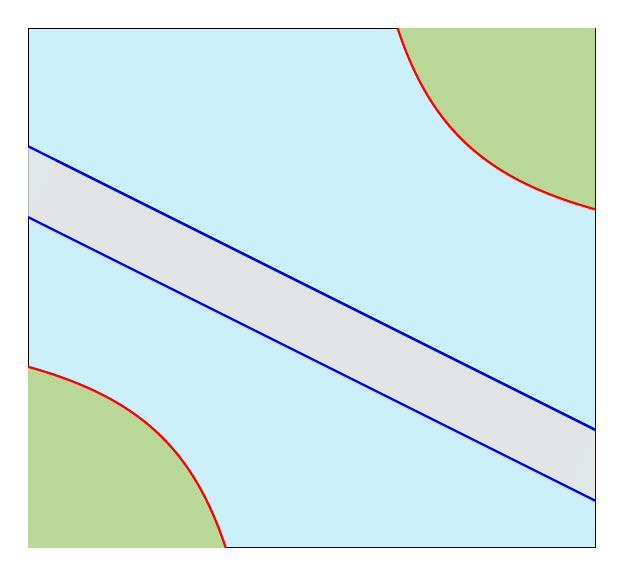
\begin{tikzpicture}[>=stealth, line cap=round, line join=round, scale=0.6]
			\definecolor{landcolor}{RGB}{185, 215, 150}
			\draw[fill=cyan!20] (-5, -4.5) rectangle (7, 6.5);
			\clip (-5, -4.5) rectangle (7, 6.5);
			\fill[gray!30, opacity=0.8] (-5, 2.5) -- (-4.4, 3.7) -- (7, -2) -- (6.4, -3.2) -- cycle;
			\fill[gray!20, opacity=0.8] 
			plot[domain=-5:7, samples=2] (\x, {-0.5*\x}) -- 
			plot[domain=7:-5, samples=2] (\x, {-0.5*\x + 1.5}) -- cycle;
			\draw[blue, thick, domain=-5:7, samples=2] plot(\x, {-0.5*\x});
			\draw[blue, thick, domain=-5:7, samples=2] plot(\x, {-0.5*\x + 1.5});
			\draw[blue, thick] (-4.4, 3.7) -- (7, -2);
			\fill[landcolor]
			(-5, -4.5) --
			plot[domain=-5:-0.8, samples=100] (\x, {(\x+9)/(\x-1)}) --
			(-1.5, -4.5) -- cycle;
			\fill[landcolor]
			(3.5, 6.5) --
			plot[domain=2.75:7, samples=100] (\x, {(\x+9)/(\x-1)}) --
			(7, 6.5) -- cycle;
			\draw[red, thick, smooth, samples=100, domain=-5:-0.8] plot(\x, {(\x+9)/(\x-1)});
			\draw[red, thick, smooth, samples=100, domain=2.75:7] plot(\x, {(\x+9)/(\x-1)});
		\end{tikzpicture}
	}
	\par
	\shortans[0]{61}
	\loigiai{
		\begin{center}
			\begin{tikzpicture}[>=stealth, line cap=round, line join=round, scale=0.6]
				\clip (-5, -4) rectangle (7.75, 6.5);
				\pgfmathsetmacro{\xMone}{1 + 2*sqrt(5)}
				\pgfmathsetmacro{\yMone}{1 + sqrt(5)}
				\pgfmathsetmacro{\xMtwo}{1 - 2*sqrt(5)}
				\pgfmathsetmacro{\yMtwo}{1 - sqrt(5)}
				\pgfmathsetmacro{\xA}{(5 + 6*sqrt(5))/5}
				\pgfmathsetmacro{\yA}{(5 - 3*sqrt(5))/5}
				\pgfmathsetmacro{\xB}{(2 - 6*sqrt(5))/5}
				\pgfmathsetmacro{\yB}{(-1 + 3*sqrt(5))/5}
				\coordinate (M1) at (\xMone, \yMone);
				\coordinate (M2) at (\xMtwo, \yMtwo);
				\coordinate (A) at (\xA, \yA);
				\coordinate (B) at (\xB, \yB);
				\coordinate (dir) at (2, -1);
				\coordinate (Aprime) at ($(A) + (dir)$);
				\coordinate (Bprime) at ($(B) - (dir)$);
				% hệ trục tọa độ
				\draw[->] (-6.5, 0) -- (7.5, 0) node[below] {$x$};
				\draw[->] (0, -4) -- (0, 6) node[left] {$y$};
				\fill (0,0) circle (1.5pt) node[below left] {$O$};
				%  đường tiệm cận
				\draw[dashed, gray] (1, -4) -- (1, 6) node[below right] {$x=1$};
				\draw[dashed, gray] (-6, 1) -- (8, 1) node[above left] {$y=1$};
				%đồ thị hàm số y = (x+9)/(x-1) 
				% Nhánh trái 
				\draw[red, smooth, samples=100, domain=-6:0.7] plot(\x, {(\x+9)/(\x-1)});
				% Nhánh phải (tránh điểm x=1)
				\draw[red, smooth, samples=100, domain=1.3:8] plot(\x, {(\x+9)/(\x-1)});
				% hai mép con đường d1 và d2
				% d1
				\draw[blue, domain=-6:8] plot(\x, {-0.5*\x}) node[right] {$d_1$};
				% d2
				\draw[blue, domain=-5:8] plot(\x, {-0.5*\x + 1.5}) node[above right] {$d_2$};
				% các đoạn thẳng khoảng cách M1A, M2B và đoạn AB
				\draw[dashed, thick] (M1) -- (A);
				\draw[dashed, thick] (M2) -- (B);
				\draw[thick, orange] (A) -- (B);
				% góc vuông
				\pic [draw, angle radius=2.5mm] {right angle = M1--A--Aprime};
				\pic [draw, angle radius=2.5mm] {right angle = M2--B--Bprime};
				% nhãn 
				\fill (M1) circle (2pt) node[above right] {$M_1$};
				\fill (M2) circle (2pt) node[below left] {$M_2$};
				\fill (A) circle (2pt) node[below] {$A$};
				\fill (B) circle (2pt) node[above] {$B$};
				
			\end{tikzpicture}
		\end{center}
		Đồ thị hàm số $(C)\colon y = \dfrac{x+9}{x-1} = 1 + \dfrac{10}{x-1}$ có đạo hàm $y' = -\dfrac{10}{(x-1)^2}$.\\
		Hai mép con đường là hai đường thẳng song song có phương trình lần lượt là $d_1\colon x+2y=0$ và $d_2\colon x+2y-3=0$.\\
		Để quãng đường bơi là ngắn nhất thì vị trí xuất phát của hai người là hai điểm $M_1$, $M_2$ thuộc hai nhánh của đồ thị $(C)$ sao cho tiếp tuyến tại đó song song với hai mép đường. Hoành độ của $M_1$, $M_2$ là nghiệm của phương trình
		\[ y' = -\dfrac{1}{2} \Leftrightarrow -\dfrac{10}{(x-1)^2} = -\dfrac{1}{2} \Leftrightarrow (x-1)^2 = 20 \Leftrightarrow \hoac{&x = 1 + 2\sqrt{5} \Rightarrow y = 1 + \sqrt{5} \\ &x = 1 - 2\sqrt{5} \Rightarrow y = 1 - \sqrt{5}.} \]
		Suy ra tọa độ hai điểm xuất phát là $M_1\left(1+2\sqrt{5}; 1+\sqrt{5}\right)$ và $M_2\left(1-2\sqrt{5}; 1-\sqrt{5}\right)$.\\
		Hai người bơi đến mép đường bằng quãng đường ngắn nhất, tức là bơi theo đường vuông góc hạ từ $M_1$, $M_2$ xuống mép đường.\\
		Từ đồ thị và phương trình đường thẳng, ta thấy nhánh chứa $M_1$ (với $x > 1$) gần với mép đường $d_2$ hơn, và nhánh chứa $M_2$ (với $x < 1$) gần với mép đường $d_1$ hơn.\\
		Gọi $A$ là hình chiếu vuông góc của $M_1$ lên $d_2$. Đường thẳng $M_1 A$ đi qua $M_1$ và vuông góc với $d_2$ nên có phương trình
		\[ 2\left(x - 1 - 2\sqrt{5}\right) - \left(y - 1 - \sqrt{5}\right) = 0 \Leftrightarrow 2x - y - 1 - 3\sqrt{5} = 0. \]
		Tọa độ điểm $A$ là nghiệm của hệ phương trình
		\[ \heva{&x + 2y - 3 = 0 \\ &2x - y - 1 - 3\sqrt{5} = 0} \Leftrightarrow \heva{&x = \dfrac{5+6\sqrt{5}}{5} \\ &y = \dfrac{5-3\sqrt{5}}{5}} \Rightarrow A\left(\dfrac{5+6\sqrt{5}}{5}; \dfrac{5-3\sqrt{5}}{5}\right). \]
		Gọi $B$ là hình chiếu vuông góc của $M_2$ lên $d_1$. Đường thẳng $M_2 B$ đi qua $M_2$ và vuông góc với $d_1$ nên có phương trình
		\[ 2\left(x - 1 + 2\sqrt{5}\right) - \left(y - 1 + \sqrt{5}\right) = 0 \Leftrightarrow 2x - y - 1 + 3\sqrt{5} = 0. \]
		Tọa độ điểm $B$ là nghiệm của hệ phương trình
		\[ \heva{&x + 2y = 0 \\ &2x - y - 1 + 3\sqrt{5} = 0} \Leftrightarrow \heva{&x = \dfrac{2-6\sqrt{5}}{5} \\ &y = \dfrac{-1+3\sqrt{5}}{5}} \Rightarrow B\left(\dfrac{2-6\sqrt{5}}{5}; \dfrac{-1+3\sqrt{5}}{5}\right). \]
		Ta có
		\[ AB^2 = \left(x_A - x_B\right)^2 + \left(y_A - y_B\right)^2 = \left(\dfrac{3+12\sqrt{5}}{5}\right)^2 + \left(\dfrac{6-6\sqrt{5}}{5}\right)^2= 37{,}8. \]
		Suy ra $AB = \sqrt{37{,}8}$.\\
		Vì đơn vị dài trên mỗi trục là $10$ mét nên khoảng cách thực tế giữa hai điểm $A$ và $B$ là
		\[ 10 \cdot AB = 10\sqrt{37{,}8} \approx 61 \text{ (m)}. \]
	}
\end{ex}

%%%============= EX_21 =============%%%
\begin{ex}%[0X0C2-9]%[TDM32]%[Nguyễn Văn Sang]
	Xếp ngẫu nhiên $36$ cuốn sách Tinh Hoa Công Phá Đề Toán giống nhau vào $18$ ngăn sách được bố trí như hình vẽ. Gọi $p$ là xác suất để thoả mãn đồng thời các điều kiện sau
	\begin{itemize}
		\item Có đúng $4$ ô để trống.
		\item Giữa hai ô trống có ít nhất $2$ ngăn có sách.
		\item Tính từ trái sang phải, giữa ô trống đầu tiên và cuối cùng có đúng $10$ ngăn sách.
	\end{itemize}
	%--- Bắt đầu vẽ hình minh hoạ đề bài ---%
	\begin{center}
		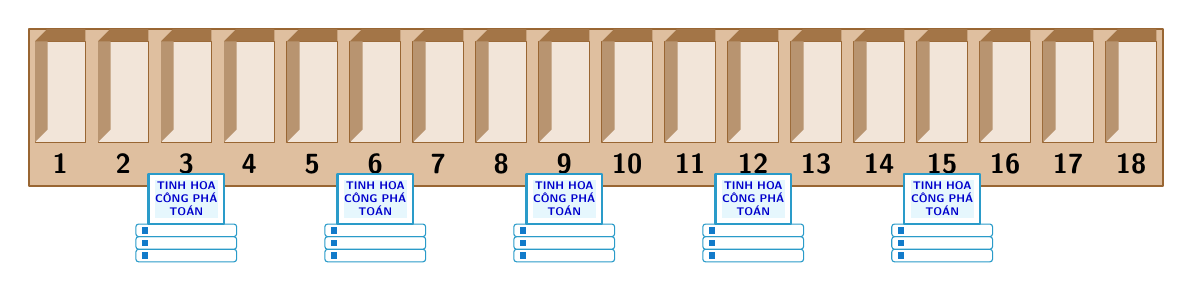
\begin{tikzpicture}[scale=0.8, font=\sffamily, line join=round]
			% Định nghĩa màu gỗ
			\colorlet{wood}{brown!50}
			\colorlet{wooddark}{brown!80!black}
			\colorlet{woodlight}{brown!20}
			
			% Khung ngoài kệ sách
			\draw[fill=wood, draw=wooddark, thick] (0,0) rectangle (18,2.5);
			
			% Các ngăn bên trong với hiệu ứng chiều sâu 3D
			\foreach \i in {0,...,17} {
				% Mặt trong ngăn
				\fill[woodlight] (\i+0.1, 0.7) rectangle (\i+0.9, 2.3);
				\draw[wooddark] (\i+0.1, 0.7) rectangle (\i+0.9, 2.3);
				% Chiều sâu bên trái
				\fill[wooddark!70] (\i+0.1, 0.7) -- (\i+0.3, 0.9) -- (\i+0.3, 2.5) -- (\i+0.1, 2.3) -- cycle;
				% Chiều sâu bên trên
				\fill[wooddark!90] (\i+0.1, 2.3) -- (\i+0.3, 2.5) -- (\i+0.9, 2.5) -- (\i+0.9, 2.3) -- cycle;
			}
			
			% Đánh số thứ tự các ngăn trên viền kệ
			\foreach \i in {1,...,18} {
				\node at (\i-0.5, 0.35) {\textbf{\i}};
			}
			
			% Các chồng sách minh hoạ xếp bên dưới kệ
			\foreach \x in {2.5, 5.5, 8.5, 11.5, 14.5} {
				% Các cuốn sách nằm ngang (chồng lên nhau)
				\foreach \y in {0, 0.2, 0.4} {
					\draw[fill=white, draw=cyan!80!black, rounded corners=1pt] (\x-0.8, -1.2+\y) rectangle (\x+0.8, -1.0+\y);
					% Gáy sách xanh
					\fill[cyan!60!blue] (\x-0.7, -1.15+\y) rectangle (\x-0.6, -1.05+\y);
				}
				% Cuốn sách dựng đứng trưng bày
				\draw[fill=white, draw=cyan!80!black, thick] (\x-0.6, -0.6) rectangle (\x+0.6, 0.2);
				\fill[cyan!10] (\x-0.5, -0.5) rectangle (\x+0.5, 0.1);
				\node[text=blue!80!black, scale=0.4, align=center] at (\x, -0.2) {\bfseries TINH HOA\\ \bfseries CÔNG PHÁ\\ \bfseries TOÁN};
			}
		\end{tikzpicture}
	\end{center}
	%--- Kết thúc vẽ hình minh hoạ ---%
	Hãy tính $10^6 p$ (\textit{làm tròn kết quả đến hàng đơn vị}).
	\par
	\shortans[0]{1919}
	\loigiai{
		\textbf{Phương pháp giải:}
		\begin{itemize}
			\item Bài toán chia kẹo Euler: Số nghiệm nguyên không âm của phương trình $x_1 + x_2 + \dots + x_k = n$ là $\mathrm{C}_{n+k-1}^{k-1}$.
			\item Số nghiệm nguyên dương của phương trình $x_1 + x_2 + \dots + x_k = n$ là $\mathrm{C}_{n-1}^{k-1}$.
			\item \textbf{Bước $1$:} Tính số phần tử của không gian mẫu $|\Omega|$ (số cách xếp $36$ cuốn sách giống nhau vào $18$ ngăn phân biệt).
			\item \textbf{Bước $2$:} Gọi biến cố $A$ là biến cố thoả mãn các điều kiện đề bài. Ta chia việc đếm số phần tử của $A$ làm hai giai đoạn:
			\begin{itemize}
				\item Chọn vị trí cho $4$ ô trống sao cho thoả mãn các khoảng cách đã cho.
				\item Xếp $36$ cuốn sách vào $14$ ô không trống còn lại (sao cho mỗi ô có ít nhất $1$ cuốn).
			\end{itemize}
		\end{itemize}
		\textbf{1. Không gian mẫu:} \\
		Xếp ngẫu nhiên $36$ cuốn sách giống nhau vào $18$ ngăn sách phân biệt. Số cách xếp chính là số nghiệm nguyên không âm của phương trình $x_1 + x_2 + \dots + x_{18} = 36$. \\
		$\Rightarrow |\Omega| = \mathrm{C}_{36+18-1}^{18-1} = \mathrm{C}_{53}^{17}$.\\
		\textbf{2. Số kết quả thuận lợi cho biến cố A:} \\
		Đánh số $18$ ngăn sách từ trái sang phải là $1, 2, \dots, 18$. \\
		Giả sử $4$ ô trống nằm ở các vị trí $e_1 < e_2 < e_3 < e_4$.
		\begin{itemize}
			\item Điều kiện \textit{\lq\lq Giữa hai ô trống có ít nhất $2$ ngăn có sách\rq\rq} suy ra 
			\[e_2 - e_1 \ge 3, \quad e_3 - e_2 \ge 3, \quad e_4 - e_3 \ge 3\]
			\item Điều kiện \textit{\lq\lq Giữa ô trống đầu tiên và cuối cùng có đúng $10$ ngăn sách\rq\rq} suy ra 
			\[e_4 - e_1 - 1 = 10 \Leftrightarrow e_4 - e_1 = 11\]
		\end{itemize}
		Mặt khác, ta có $(e_4 - e_3) + (e_3 - e_2) + (e_2 - e_1) = e_4 - e_1 = 11$. \\
		Đặt $d_1 = e_2 - e_1$, $d_2 = e_3 - e_2$, $d_3 = e_4 - e_3$, ta có hệ
		\[ \heva{& d_1 + d_2 + d_3 = 11 \\ & d_1 \ge 3, d_2 \ge 3, d_3 \ge 3} \]
		Đặt $x_1 = d_1 - 3$, $x_2 = d_2 - 3$, $x_3 = d_3 - 3$ (với $x_i \ge 0, \forall i \in \{1; 2; 3\}$). \\
		Phương trình trở thành $x_1 + x_2 + x_3 = 11 - 9 = 2$. \\
		Số nghiệm nguyên không âm của phương trình này là $\mathrm{C}_{2+3-1}^{3-1} = \mathrm{C}_4^2 = 6$ cách. \\
		Khối gồm $4$ ô trống và các ô có sách nằm sát giữa chúng có tổng chiều dài là $e_4 - e_1 + 1 = 12$ ô.\\ 
		Khi xếp khối dài $12$ ô này vào $18$ ngăn, vị trí bắt đầu $e_1$ có thể trượt từ vị trí $1$ đến vị trí $18 - 12 + 1 = 7$. Do đó, có $7$ cách tịnh tiến chọn $e_1$. \\
		$\Rightarrow$ Số cách chọn vị trí cho $4$ ô trống là $6 \cdot 7 = 42$ cách.\\
		Sau khi đã cố định được $4$ ô trống, ta còn lại $14$ ô có sách. Tiếp tục xếp $36$ cuốn sách giống nhau vào $14$ ô này sao cho mỗi ô có ít nhất $1$ cuốn. Số cách xếp bằng số nghiệm nguyên dương của phương trình $y_1 + y_2 + \dots + y_{14} = 36$. \\
		Số cách phân phối sách là $\mathrm{C}_{36-1}^{14-1} = \mathrm{C}_{35}^{13}$ cách. \\
		Suy ra, số kết quả thuận lợi của biến cố $A$ là $|A| = 42 \cdot \mathrm{C}_{35}^{13}$.
		%--- Hình minh hoạ tư duy xếp vách ngăn ---%
		\begin{center}
			\begin{tikzpicture}[xscale=0.85, yscale=0.8, font=\footnotesize]
				% Draw the main bookshelf grid for logic explanation
				\draw[thick] (0,0) rectangle (18, 1.2);
				\foreach \i in {1,...,17} {
					\draw[thick] (\i,0) -- (\i,1.2);
				}
				% Numbering
				\foreach \i in {1,...,18} {
					\node at (\i-0.5, -0.4) {\i};
				}
				% Shade empty compartments (e.g., valid example: 2, 5, 8, 13)
				\foreach \i in {2, 5, 8, 13} {
					\fill[red!15] (\i-1, 0.05) rectangle (\i, 1.15);
					\node[red, font=\bfseries] at (\i-0.5, 0.6) {Trống};
				}
				% Non-empty compartments
				\foreach \i in {1, 3, 4, 6, 7, 9, 10, 11, 12, 14, 15, 16, 17, 18} {
					\node[blue] at (\i-0.5, 0.6) {$\ge 1$};
				}
				
				% Braces for distance
				\draw[thick, blue] (2, 1.3) -- (2, 1.5) -- (12, 1.5) -- (12, 1.3);
				\node[blue, above] at (7, 1.5) {Đúng $10$ ngăn sách nằm giữa ô trống đầu và cuối};
				
				% Braces for spaces between empty cells
				\draw[thick, teal] (2, -0.8) -- (2, -1) -- (4, -1) -- (4, -0.8);
				\node[teal, below] at (3, -1) {$\ge 2$ ngăn};
				
				\draw[thick, teal] (5, -0.8) -- (5, -1) -- (7, -1) -- (7, -0.8);
				\node[teal, below] at (6, -1) {$\ge 2$ ngăn};
				
				\draw[thick, teal] (8, -0.8) -- (8, -1) -- (12, -1) -- (12, -0.8);
				\node[teal, below] at (10, -1) {$\ge 2$ ngăn};
				
			\end{tikzpicture}
		\end{center}
		\textbf{3. Tính xác suất:} \\
		Xác suất của biến cố là $\mathrm{P}(A) = \displaystyle \dfrac{n(A)}{n(\Omega)} = \dfrac{42 \cdot \mathrm{C}_{35}^{13}}{\mathrm{C}_{53}^{17}}\approx 0{,}00191917$. \\
		Giá trị cần tìm là $10^6 \cdot \mathrm{P}(A) \approx 1\,919$.
	}
\end{ex}

%%%============= EX_22 =============%%%
\begin{ex}%[2D4C1-4]%[TDM32]
	Ở một hội trường có tất cả $N_0$ người đang bắt đầu tranh luận về một vấn đề bảo tồn di sản văn hoá và giả sử chỉ có ba nhóm là: tán thành, phản đối và trung lập. Ở thời điểm ban đầu số người tán thành và phản đối lần lượt là $30$ và $40$, cả hai nhóm này đều tiến hành thuyết phục và lôi kéo nhóm trung lập. Biết rằng tốc độ tăng số lượng thành viên của nhóm tán thành tỉ lệ thuận với số lượng hiện có của nhóm trung lập theo hệ số $\dfrac{1}{2}$ và tốc độ tăng số lượng thành viên của nhóm phản đối tỉ lệ nghịch với số lượng thành viên của nhóm trung lập. Sau $1$ giờ nhóm tán thành và phản đối có số lượng thành viên là $40$ và $46$, sau $2$ giờ thì số lượng của hai nhóm này tương ứng là $50$ và $49$. Biết rằng $\left\{[N(t)]^2\right\}' = 2N(t) \cdot N'(t)$ và $\left\{\mathrm{e}^t N(t)\right\}' = \mathrm{e}^t \left[N(t) + N'(t)\right]$. Hãy xác định $N_0$ (\textit{làm tròn kết quả đến hàng đơn vị}).
	\par
	\shortans[0]{104}
	\loigiai{
		Gọi $X(t), Y(t), F(t)$ lần lượt là số lượng người của nhóm tán thành, nhóm phản đối và nhóm trung lập sau $t$ giờ ($t \ge 0$). \\
		Tại mọi thời điểm, tổng số người không đổi nên ta có
		\[ X(t) + Y(t) + F(t) = N_0 \Rightarrow F(t) = N_0 - X(t) - Y(t). \]
		Đạo hàm hai vế theo $t$, ta được 
		\[ X'(t) + Y'(t) + F'(t) = 0 \Rightarrow F'(t) = -X'(t) - Y'(t). \]
		Theo giả thiết bài toán, tốc độ tăng của nhóm tán thành và phản đối lần lượt thoả mãn
		\[ \heva{& X'(t) = \dfrac{1}{2} F(t) \\ & Y'(t) = \dfrac{k}{F(t)}} \quad (k \text{ là hằng số tỉ lệ}). \]
		Thay vào phương trình của $F'(t)$ ta có
		\[ F'(t) = -\dfrac{1}{2} F(t) - \dfrac{k}{F(t)}. \]
		Nhân cả hai vế với $2F(t)$ để khử mẫu
		\[ 2F(t) \cdot F'(t) = -[F(t)]^2 - 2k \Leftrightarrow \big[ (F(t))^2 \big]' + \big[ F(t) \big]^2 = -2k. \]
		Nhân cả hai vế với $\mathrm{e}^t$
		\[ \mathrm{e}^t \big[ (F(t))^2 \big]' + \mathrm{e}^t \big[ F(t) \big]^2 = -2k \mathrm{e}^t. \]
		Áp dụng công thức $\left\{\mathrm{e}^t N(t)\right\}' = \mathrm{e}^t \left[N(t) + N'(t)\right]$ được gợi ý ở đề bài, ta có
		\[ \left( \mathrm{e}^t \cdot \big[ F(t) \big]^2 \right)' = -2k \mathrm{e}^t. \]
		Lấy nguyên hàm hai vế theo biến $t$:
		\[ \mathrm{e}^t \cdot \big[ F(t) \big]^2 = \int -2k \mathrm{e}^t \mathrm{\,d}t \Rightarrow \mathrm{e}^t \cdot \big[ F(t) \big]^2 = -2k \mathrm{e}^t + C \Rightarrow \big[ F(t) \big]^2 = C \mathrm{e}^{-t} - 2k \quad (*). \]
		Khai thác các dữ kiện bài toán tại $t=0, t=1, t=2$:
		\begin{itemize}
			\item Tại $t=0$: $X(0) = 30$, $Y(0) = 40 \Rightarrow F(0) = N_0 - 30 - 40 = N_0 - 70$.
			\item Tại $t=1$: $X(1) = 40$, $Y(1) = 46 \Rightarrow F(1) = N_0 - 40 - 46 = N_0 - 86$.
			\item Tại $t=2$: $X(2) = 50$, $Y(2) = 49 \Rightarrow F(2) = N_0 - 50 - 49 = N_0 - 99$.
		\end{itemize}
		Thay các giá trị này vào $(*)$, ta được hệ phương trình
		\[ \heva{& (N_0 - 70)^2 = C - 2k \quad &(1) \\ & (N_0 - 86)^2 = C \mathrm{e}^{-1} - 2k \quad &(2) \\ & (N_0 - 99)^2 = C \mathrm{e}^{-2} - 2k \quad &(3)} \]
		Lấy $(2)$ trừ $(1)$ vế theo vế, ta được
		\[ (N_0 - 86)^2 - (N_0 - 70)^2 = C(\mathrm{e}^{-1} - 1) \Leftrightarrow -32N_0 + 2\,496 = C(\mathrm{e}^{-1} - 1) \quad (4). \]
		Lấy $(3)$ trừ $(2)$ vế theo vế, ta được
		\[ (N_0 - 99)^2 - (N_0 - 86)^2 = C(\mathrm{e}^{-2} - \mathrm{e}^{-1}) = C \mathrm{e}^{-1}(\mathrm{e}^{-1} - 1) \Leftrightarrow -26N_0 + 2\,405 = C \mathrm{e}^{-1}(\mathrm{e}^{-1} - 1) \quad (5). \]
		Lấy $(5)$ chia $(4)$ vế theo vế
		\begin{align*}
			&\dfrac{-26N_0 + 2\,405}{-32N_0 + 2\,496} = \mathrm{e}^{-1} = \dfrac{1}{\mathrm{e}} \\
			\Leftrightarrow \ & \mathrm{e}(-26N_0 + 2\,405) = -32N_0 + 2\,496 \\
			\Leftrightarrow \ & N_0 (32 - 26\mathrm{e}) = 2\,496 - 2\,405\mathrm{e} \\
			\Leftrightarrow \ &N_0 = \dfrac{2\,405\mathrm{e} - 2\,496}{26\mathrm{e} - 32} \approx 104.
		\end{align*}
	}
\end{ex}
